\documentclass[11pt]{standalone}

\usepackage{ifthen}
\usepackage{amsmath}
\usepackage{tikz} 

\usepackage[d]{esvect}
\usetikzlibrary{shapes.misc}
\usetikzlibrary{arrows,arrows.meta}
\usetikzlibrary{calc,intersections, patterns, math}

\definecolor{pfeil}{RGB}{168,167,167}
\definecolor{salmon}{RGB}{250,128,114}
\definecolor{petrol}{RGB}{0, 118, 136}
\definecolor{darkgoldenrod}{RGB}{184, 134, 11}
\colorlet{petrol-lighter}{petrol!40}
\colorlet{darkgoldenrod-lighter}{darkgoldenrod!40}

\begin{document}

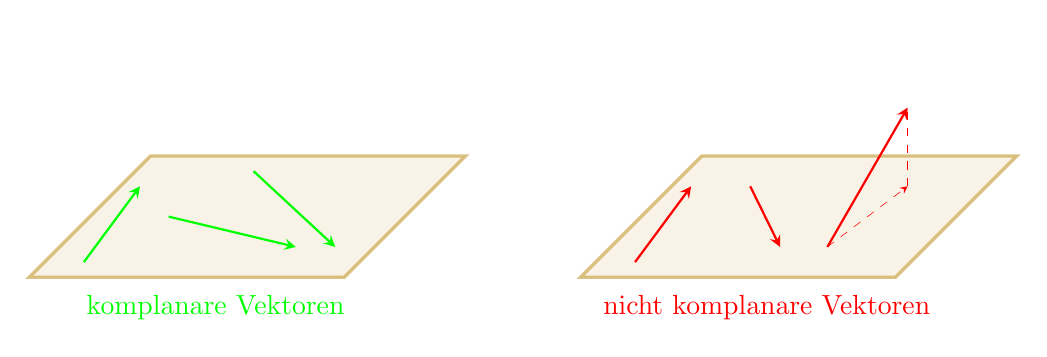
\begin{tikzpicture}[pfeil, >=stealth, very thick,
	% line join=round,
    % line cap=round,
    rotate around x=-90,
    rotate around z=-90,
]

% Achsen
\draw[->,thick,transparent]   (0,0,0) -- (2,0,0) node[below left]{$x$};
\draw[->,thick,transparent] (0,0,0) -- (0,2,0) node[below right]{$y$};
\draw[->,thick,transparent]  (0,0,0) -- (0,0,2) node[above]{$z$};

\draw[darkgoldenrod, fill=darkgoldenrod!20, opacity=0.5] (2,2,0) -- (2,-2,0) -- (-2,-2,0) -- (-2,2,0) -- cycle;

\draw[green, ->, thick] (1.5,-1.5,0) -- (-1,-1.75,0);
\draw[green, ->, thick] (-1.5,-0.5,0) -- (1,1.5,0);
\draw[green, ->, thick] (0,-1,0) -- (1,1,0);

\node[green] at (3,0.75,0) {komplanare Vektoren};


\begin{scope}[shift={(0,7,0)}]
\draw[->,thick,transparent]   (0,0,0) -- (2,0,0) node[below left]{$x$};
\draw[->,thick,transparent] (0,0,0) -- (0,2,0) node[below right]{$y$};
\draw[->,thick,transparent]  (0,0,0) -- (0,0,2) node[above]{$z$};

\draw[darkgoldenrod, fill=darkgoldenrod!20, opacity=0.5] (2,2,0) -- (2,-2,0) -- (-2,-2,0) -- (-2,2,0) -- cycle;

\draw[red, ->, thick] (1.5,-1.5,0) -- (-1,-1.75,0);
\draw[red, <-, thick] (1,0.15,0) -- (-1,-1,0);

\draw[red, ->, thick] (1,0.75,0) -- (-1,1,1);
\draw[red, -, very thin, dashed] (-1,1,0) -- (-1,1,1);
\draw[red, ->, very thin, dashed] (1,0.75,0) -- (-1,1,0);


\node[red] at (3,0.75,0) {nicht komplanare Vektoren};
\end{scope}


\end{tikzpicture}

\end{document}

